\chapter{Conclusion}

\section{Useful features in Intrusion Detection}

\paragraph{}
It is evident from this study that the basic features, such as source to destination time to live, destination to source time to live and state of the data packet are few of the most important features for intrusion detection. However, relying on them completely may lead to a system which may not respond to growing trends in cyber security. This may be because most of the attacks classified in UNSW-NB15 dataset use exploits related to these basic features. If other features are completely ignored and attackers figure out ways to exploit those features, it will become impossible to detect those intrusions in the future. It is important to update the list of important features by running periodic tests overr fresh data.

\section{Notes about the different models}

\paragraph{}
A few interesting cases came up durnig the tests.
\begin{itemize}
    \item The GaussianNB classifier, when tested with all features, had the lowest execution time, and the lowest accuracy. It may be because GaussianNB works under the assumption that the features are not related to each other. There is minimal computation resulting in lower time signatures and since the assumption is not realistic, the accuracy might have suffered. When tested with the 2 selected features, however, while the execution time remained comparable to other models, the accuracy increased significantly. This increase in accuracy may be attributed to the low dimensionality of the dataset with just 2 features making the assumption more realistic than before.
    \item Decision Tree classifier with max-depth 2, gave the exact same predictions when tested with all features and when tested with 2. This may be because the optimization done with the feature selection is used automatically by the Decision Tree algorithm. The extra time used with all features must be due to the process of selecting these features. Since there are only 2 features which are selected, max-depth of 2 gives an optimal classification result. (Figure \ref{dtc_md2_2_features})
\end{itemize}

\begin{figure}[h]
    \hfill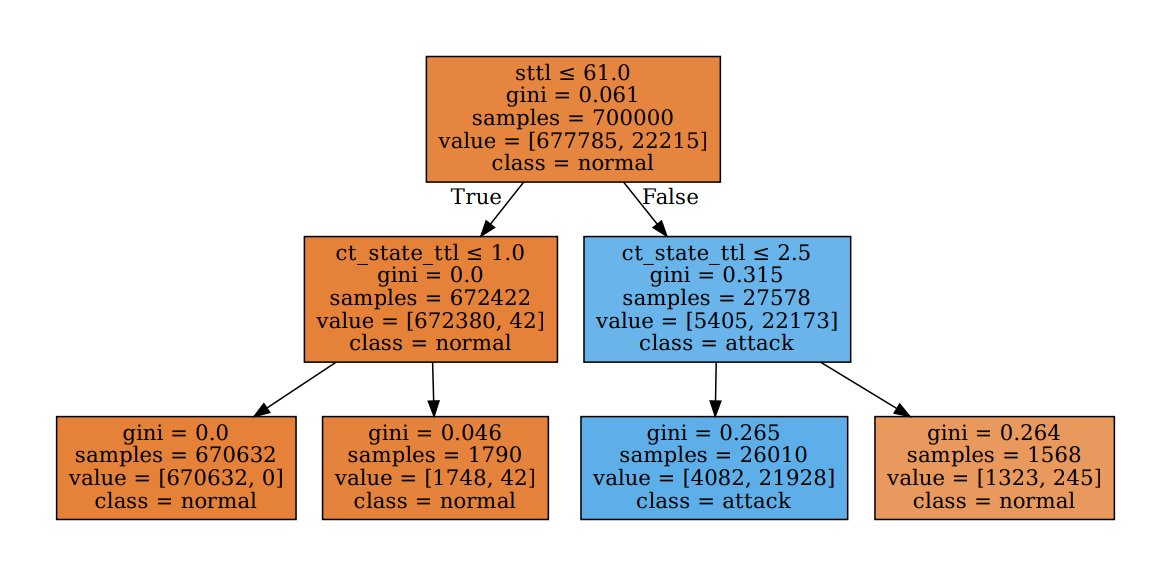
\includegraphics[width=1\textwidth]{Chapter5/dtc_md2_2_features}\hspace*{\fill}
    \caption{Decision Tree with max-depth = 2 tested with 2 features}
    \label{dtc_md2_2_features}
\end{figure}

\section{Scope}

\paragraph{}
Given that the UNSW-NB15 is a realistic dataset, the results from these models suggest Decision Trees as the most optimal model to implement an IDS in a low powered environment. More tests must be conucted to find an optimal value for the internal parameters of Decision Trees, such as max-depth. The radical improvement in performance from the two selected features is very convincing, however choosing the right features will be dependant on the type of data going in as input into the system and the way they are distibuted. The correct features may vary from network to network, and extreme care must be taken while implementing such a model.

\paragraph{}
Tests must be conducted on live data and small devices, which are the focus of this work. The results from this work may act as a starting point to further research in this domain.
